\documentclass[a5paper]{article} 
%\usepackage{amsmath,amsthm,amsfonts}
\usepackage[bulgarian]{babel}
\usepackage[numbers]{natbib}
\usepackage{rotating}
\usepackage{amsfonts,amsmath,amsthm}
\usepackage{graphicx}
\usepackage{color} 
%\usepackage[notref,notcite]{showkeys}
\usepackage{multirow}
\usepackage[utf8]{inputenc}
\usepackage[T2A]{fontenc}
%\usepackage[outdir=./]{epstopdf}
\usepackage{epstopdf}
\usepackage{wrapfig}
\usepackage{placeins}
\usepackage[left=1.5cm,bottom=1.5cm,top=1cm,right=1cm]{geometry}
%\usepackage[colorlinks=false, urlcolor=blue]{hyperref}
%\usepackage[ sorting=none ]{biblatex}
%    natbib=true,
%    style=numeric,

\newcommand{\be}{\begin{equation}}
\newcommand{\ee}{\end{equation}}
\newcommand{\rf}[1]{(\ref{#1})}
\newcommand{\RR}{\mathbb{R}}
\newtheorem{thm}{Theorem}
\newtheorem{lm}{Lemma}

\newcommand{\eeth}{\rm}
\newcommand{\dO}{\partial\Omega_{h}}
\theoremstyle{remark}
\newtheorem*{remark}{Remark}

\begin{document}
\begin{large}

%titlepage
%\thispagestyle{empty}
\begin{center}
%University logo
\begin{figure}[!htb]
      
\includegraphics[width=1\linewidth]{LogoThesis.png}
\end{figure}

\begin{minipage}{0.95\linewidth}
    \centering
    \vspace{0.5cm}
%Thesis title
    {\Large ЧИСЛЕНО ИЗСЛЕДВАНЕ НА\\ ДВУМЕРНОТО УРАВНЕНИЕ НА БУСИНЕСК\par}
    \vspace{2cm}
%Author's name
    {\Large Красимир Андреев Ангелов \par с научен ръководител \\проф. д-р Наталия Кольковска\par}
    \vspace{2cm}
    {\Large АВТОРЕФЕРАТ\par}
    \vspace{1cm}
%Degree
    {\large на дисертация за присъждане на образователна и научна степен ``Доктор по математика'' със специалност ``Математическо моделиране и приложение на математиката''\par}
    \vspace{3cm}
%Date
    {\Large Януари 2023}
\end{minipage}
\end{center}
\clearpage

\shipout\null
%\stepcounter{page}


\tableofcontents
\newpage

%\begin{appendix}
%  \listoffigures
%  \listoftables
%\end{appendix}

\section{Въведение}\label{introduction}
Настоящият труд разглежда моделна задача, описваща поведението на самотна вълна в плитки води, движеща се в правоъгълен канал. Математическият модел е открит първоначално от Джоузеф Бусинеск, важи за дълги нелинейни вълни и е известен с това, че нелинейността и дисперсията изпадат в самобалансиращо се състояние \cite{ref01,ref02}. Проф. Христо Христов \cite{ref1} извежда клас от вълнови уравнения, базирани на предходните две работи и едно от тях е наречено ``Парадигматично уравнение на Бусинеск'' (ПУБ):
\begin{align}
&u_{tt} - \Delta u -\beta_1  \Delta u_{tt} +\beta_2 \Delta ^2 u + \Delta f(u)=0   \quad \text{при} \;  (x,y) \in \RR^2, \, t\in\RR^+,\label{eq1}
\\ \nonumber &u(x,y,0)=u_0(x,y), \, u_t(x,y,0)=u_1(x,y)   \quad\text{при} \; (x,y) \in \RR^2,
\\  &u(x,y) \rightarrow 0,  \Delta u(x,y) \rightarrow 0 ,  \quad \text{при}  \sqrt{x^2 + y^2} \rightarrow \infty, \label{eq11}
\end{align}
където $f(u)=\alpha u^2$, $\alpha>0$ е амплитудата, $\beta_1>0$, $\beta_2>0$ са дисперсионни параметри, а $\Delta$ е операторът на Лаплас. Показано е, че уравнението \rf{eq1} е частично интегруемо и са изведени три закона за запазване на енергията, масата и момента \cite{ref1, ref159}. Други инварианти не са ми известни. 

Задачата \rf{eq1}-\rf{eq11} и численото ѝ решение ще са основна цел на настоящата работа. Уравненията на Бусинеск се използват не само за изучаване на динамиката на така наречените дълги вълни в плитка водна среда (например канал). Те могат да моделират разпространението на вълни в еластичен прът или в непрекъснатия еквивалент на решетъчни структури на молекулно ниво.

Началото на тази работа се фокусира върху решения на \rf{eq1} от вида 
\be\label{sub123}
u(x,y,t)=U(x,y-ct),
\ee
които са стационарни солитонни вълни (ССВ), движещи се по $y$ оста със скорост $c$. След полагане на \rf{sub123} в \rf{eq1}, ССВ удовлетворяват следното нелинейно елиптично диференциално уравнение от четвърти ред
\begin{equation}\label{eq2}
c^2 (E_1-\beta_1 \Delta) U_{yy} = \Delta U -\beta_2 \Delta^2 U - \Delta f(U),
\end{equation}
където $E_1$ е тъждествения оператор, при условие че $c < c_{max}:=\min (\sqrt{\beta_2}/ \sqrt{\beta_1},1)$. В последствие тези вълни ще служат за начално условие на хиперболичното уравнение \rf{eq1} -- \rf{eq11}. 

Алгебричните изрази от \cite{ref15}, които апроксимират решението на елиптичното уравнение \rf{eq2}, са използвани като начално условие за числени симулации на ПУБ \rf{eq1} -- \rf{eq11}, 
(виж  \cite{ref21, ref20, ref23, ref22, ref24}). Първите четири статии показват, че при стойности на скоростта $c \le 0.3$, ССВ се разсейват във формата на разширяваща се пръстеновидна вълна или избухват след кратък период от време. В последния труд \cite{ref24} са направени експерименти при по високи скорости $c=0.5,0.6$, 
но отново резултатите за формата на вълната са сходни с вече документираното поведение. 
Вижда се, че балансът между дисперсията и нелинейността в ПУБ \rf{eq1} е много крехък, 
което изисква повече усилия при запазването му. 

Едномерното ПУБ
\begin{align}
&u_{tt} - u_{xx} -\beta_1  u_{ttxx} +\beta_2 u_{xxxx} + f(u)_{xx}=0   \quad \text{при} \,  x \in \RR, \, t\in\RR^+,\label{eq1D}
\\ \nonumber &u(x,0)=u_0(x), \, u_t(x,0)=u_1(x)   \quad\text{при} \, x \in \RR,
\\  &u(x) \rightarrow 0,  u(x)_{xx} \rightarrow 0 ,  \quad \text{при} \, x \rightarrow \infty, \label{eq1d1}
\end{align}
притежава точно решение от тип солитон при $u =\tilde u(x-ct)$:
\begin{align}
\tilde u(x,t:c) = \frac{3}{2} \frac{c^2-1}{\alpha}sech^2 \left( \frac{1}{2}  \sqrt{ \frac{\beta_1 (c^2-1)}{\beta_1 c^2-\beta_2}} (x-c t \sqrt{\frac{\beta_1}{\beta_2}} ) \right).
\end{align}
Солитон е бягаща със скорост $c$ вълна от вида $\phi(x-ct)$, която е локализирана в пространството и при движение запазва формата си. Структурата ѝ се запазва дори след взаимодействие с друг(и) солитон(и).

Също така е добре известно, 
че при числени симулации в едномерния случай, за уравнение \rf{eq1D}, при условие, че $\beta_1/\beta_2 \le 1$ солитонните вълни са нестабилни за малки скорости $c$ около нулата и стабилни за 
по-големи скорости, както е показано в \cite{ref10000}. В последствие, такива изследвания са направени и за многомерното ПУБ, при $\beta_1/\beta_2 = 1$ (виж \cite{ref1c0}), където е изведено необходимо условие за скоростта, спрямо критичната енергия, при което вълната е устойчива.

Тези наблюдения изместват фокуса към изчисляване на ССВ от \rf{eq1} с по-голяма точност и при по-големи скорости $c \approx c_{max}$, тъй като това е от съществено значение за конструирането на началните данни за ПУБ \rf{eq1}-\rf{eq11}. Важно е да получим числено решение на \rf{eq2} с висока точност, чрез гъвкав и устойчив процес, който ще позволи тестването на повече и различни сценарии за развитие на решенията на хиперболичната задача \rf{eq1}-\rf{eq11}.

\subsection{Литературен обзор}
Предисторията на изчисляването на ССВ за уравнение \rf{eq1} е свързана с няколко числени техники, както следва - спектрален метод на Гальоркин е изполван в \cite{ref14,ref13}; метод на простата итерация и шаблони с крайни разлики от втори порядък върху неравномерна мрежа са приложени в \cite{ref117,ref116}; пертурбационно решение с развитие в ред около малък параметър (скоростта $c$) е представено в \cite{ref15}, където са изведени така наречените ``best-fit'' апроксимационни формули. Освен това в \cite{ref159} са изведени аналогични формули с тези от \cite{ref15}, но за нелинейност от вида $\alpha(u^3 - \sigma u^5)$.

Следните резултати се отнасят за двумерното ПУБ.
Христов, Кольковска и Василева \cite{ref20} разработват метод с неявна консервативна схема и неравномерна мрежа. Василева и Кольковска \cite{ref200} представят числен метод с движеща се координатна система. Черток, Христов и Курганов \cite{ref21} трансформират ПУБ в система от хиперболично и елиптично уравнения. При първото е използвана консервативна схема на Годунов, а за второто е приложен числен метод за елиптични уравнения базиран на бързи преобразувания на Фурие върху равномерна мрежа. В статията \cite{ref241} на Димова и Кольковска е изведена консервативна схема, където пространственият оператор пред втората производна по времето е разложен на произведение от три дискретни такива, което води до решаване на пет-диагонални системи от линейни уравнения. В \cite{ref23} Димова и Василева сравняват числения метод от \cite{ref241} с друга консервативна схема приложена върху системата показана в \cite{ref21}, при равномерна и неравномерна мрежи, като решенията от двата подхода си съответстват едно на друго. Кольковска \cite{ref25, ref251, ref252} е извела класове от трислойни и четирислойни консервативни диференчни схеми както с, така и без вътрешни итерации (на Пикард). Схемите без вътрешни итерации се изпълняват по-бързо. Блинков, Гердт, Панкратов и Коткова \cite{ref253} представят нова неявна консервативна схема, базирана на комбинацията от метод на крайните обеми и числено интегриране. Всички тези статии \cite{ref20, ref21, ref241, ref23, ref25, ref251, ref252, ref253} апроксимират вторите производни в уравнение \rf{eq1} с крайни разлики от втори ред - $O(|h|^2 + \tau^2)$. Кольковска и Ангелов \cite{ref22} използват векторни схеми на Абрашин върху равномерна мрежа. На всеки слой по времето се получават по две числени апроксимации за решението като втората "изглажда" първата с грешки от апроксимациите $O(|h|^2 + \tau)$. В \cite{ref24}, Юю Хе и Хонгтао Чен, извеждат неявна компактна консервативна схема с грешки $O(|h|^4 + \tau^2)$. Числените резултати са направени върху равномерна мрежа. Вучева и Кольковска \cite{ref254} прилагат вариация на Рунге-Кута схеми за получаване на симплектични числени методи с грешки $O(|h|^2 + \tau^4)$. 

Всичките статии, изброени в тази част, които представят числени решения на двумерното Парадигматично уравнение на Бусинеск (някои от статиите представят метод за многомерното ПУБ, но резултати само за едномерната задача), имат поне един пример с начално условие от \cite{ref15}, т.е. ``best-fit'' формулите. Разбира се са използвани и други, но нито една от тези работи не представя резултати с начално условие получено чрез итерационен подход за решаване на съответното елиптично уравнение \rf{eq2} (напр. ``Метод на Якоби'', ``Метод на простата итерация" и т.н.). Входни данни, (т.е. $u_0(x,y)$ и $u_1(x,y)$ от \rf{eq1}-\rf{eq11}) получени с такъв алгоритъм (наречен още ``False Transients''), са разработени от Христов и Чаудури в \cite{ref117,ref116}. Въпреки това все още липсват диференчни схеми от четвърти и по висок порядък $O(|h|^p)$, $p \ge 4$ за решаване на елиптичното стационарно уравнение на Бусинеск. В допълнение, все още няма разработени диференчни схеми за двумерното Парадигматично уравнение на Бусинеск с четвърти и по-висок порядък на апроксимация на вторите производни, едновременно по пространството и времето $O(|h|^p + \tau^p)$, $p \ge 4$.
%\iffalse

\subsection{Цели на дисертацията}
Основната цел на този труд е да покаже, че двумерното ПУБ притежава числени решения със свойства на солитон. Построяването на подходящо начално условие заема съществена част от изследването на ПУБ и води до решаване на друга задача - стационарното (елиптично) уравнение на Бусинеск. Подробното изследване на тези две уравнения поставят следните цели:
\begin{itemize}
  \item построяване на диференчни схеми с висок ред на апроксимация (втори, четвърти и шести) върху равномерна мрежа за решаването на двумерните стационарно и хиперболично уравнения на Бусинеск;
  \item изследване на измененията в свойствата (енергията, масата, максимума и формата) на численото решение в зависимост от реда на апроксимация;
  \item сравнение между численото решение, получено за елиптичната задача, и ``best-fit'' формулите от Пертурбационното решение на проф. Христов \cite{ref15};
  \item построяване на ново асимптотично гранично условие за решаването на елиптичната задача;
  \item изследване на числените решения на хиперболичното уравнение \rf{eq1} при по-високи скорости $c$ близки до допустимия максимум $c \approx \min (\sqrt{\beta_2}/ \sqrt{\beta_1},1)$, $c < \min (\sqrt{\beta_2}/ \sqrt{\beta_1},1)$ с начално условие, получено от численото решение на елиптичната задача \rf{eq2} (построено с метода на простата итерация);
  \item сравнение между числените резултати, получени с метода на Тейлор и други известни в литературата решения, използващи консервативни схеми (виж \cite{ref20, ref23}) с втори ред на апроксимация на вторите производни за хиперболичната задача.
\end{itemize}

\section{Съдържание на дисертацията}
 
\textbf{Глава 2. Основни числени инструменти}

В тази глава са дефинирани помощни средства и алгоритми, които се използват при численото решение на двумерните стационарно и хиперболично уравнения на Бусинеск. Дискретизацията на пространствената област $\Omega_h$ е дефинирана чрез:
\begin{align}\label{Omega}
\Omega_h = \{(x_i,y_j):& x_i = (i-\frac{N_x-1}{2})h, \; y_j = (j-\frac{N_y-1}{2})h, \nonumber\\
                                   & i = 0,\cdots, N_x-1, j = 0 ,\cdots , N_y-1 \},
\end{align}
където $N_x$ и $N_y$ описват броят точки по осите $x$ и $y$. Стъпката по пространството $h$ удовлетворява $h =2 L_x/(N_x-1) =2 L_y/(N_y-1)$, където $2 L_x$ и $2 L_y$ са размерите на областта $\Omega$. Дискретният времеви интервал е дефиниран аналогично чрез
\be
T_{\tau} = \{(t_k): t_k = k\tau, k = 0,\cdots ,N_t-1 \},
\ee
където $N_t$ е броят точки по оста $t$, а $\tau = T/(N_t-1)$ е стъпката по времето.

За дискретизация на оператора на Лаплас са използвани централни крайни разлики с различна степен на апроксимация:
\begin{equation}\label{fdx}
u_{\widehat{xx},p}(x,y) :=  \frac{1}{h^2} \sum\limits_{i=-p/2}^{p/2} d_i u(x+ih, y_j), \; p=2,4,6.
\end{equation}
като теглата $d_i$ са взети от \cite{forn} и са описани в Таблица \ref{table:A00}. Производните по $y$ се дефинират аналогично.

\begin{table}[ht]
\centering
\small
		\begin{tabular}{||c|l|l|l|l|l|l|l||}
			\hline
			\hline
            $p=2$          &          &                                 &     1      &   -2   &    1    &    &        \\
   			\hline 
			\hline 
           $p=4$          &                            &   $-\frac{1}{12}$     &     $\frac{4}{3}$      &   $-\frac{5}{2} $     &    $\frac{4}{3}$    &  $-\frac{1}{12}$   &        \\
	   \hline
			\hline 
            $p=6$        &   $\frac{1}{90}$       &     $-\frac{3}{20}$     &    $\frac{3}{2}$      &    $-\frac{49}{18}$   &    $\frac{3}{2}$    & $-\frac{3}{20}$    &    $\frac{1}{90}$       \\
	   \hline
			\hline 
		\end{tabular}
	\caption{Централни крайни разлики, използвани при апроксимацията на оператора на Лаплас.}
	\label{table:A00}
\end{table}
Грешката от дискретните апроксимации \rf{fdx} е $O(h^p)$ в зависимост от избора на $p$.

Редът на сходимост на изследваните крайни разлики и развития в ред на Тейлор са получени посредством правилото на Рунге:
\begin{equation}\label{Runge}
\xi = ln  \frac{\Vert u_{h,\tau} - u_{(h/2,\tau/2)} \Vert_\kappa } {\Vert  u_{(h/2,\tau/2)} - u_{(h/4,\tau/4)} \Vert_\kappa  } / ln(2),
\end{equation}
когато не е известно аналитично решение на уравнението, а нормата $\kappa$ е подходящо подбрана. Тук $u_{h,\tau}$ е решението получено при стъпки $h$ и $\tau$. В настоящата работа за $\kappa$ са използвани $L_2$ и $L_\infty$ норми:
\begin{align*}
\Vert u_{h,\tau} \Vert_{L_2} = \sqrt{ h^2 \sum_{i=1}^{N_x-1} \sum_{j=1}^{N_y-1}  (u_{i,j})^2 } \\
\Vert u_{h,\tau} \Vert_{\infty} = \max_{i,j}(|u_{i,j}|), \; i=1,..,N_x, j=1,..,N_y
\end{align*}

Числените резултати, получени при намиране на решенията на елиптичната и хиперболичната задачи, са извършени при $\alpha = 1$ и следните три случая : $\beta = 3$, $c=0.45$ (Тест 1), $\beta = 1$, $c=0.9$ (Тест 2) и $\beta = 3$, $c=0.3$ (Тест 3) с последващи уточнения. Първо, Консервативната схема е имплементирана само при $p=2$. Второ, при хиперболичната задача стъпката по времето е $\tau = h/2$. Трето, при решаването на елиптичната задача се използва мрежата $\omega_h \subset \Omega_h$ само в първи квадрант, като там се прилага симетричното гранично условие по абцисата и ординатата, докато хиперболичната задача се разглежда в цялата област $\Omega_h$ и там не се използва симетричното, а само нулево гранично условие.

Извели сме три различни квадратурни формули за пресмятане на интеграли, които са подробно описани в \cite{refHyp}. Тези формули са използвани за пресмятане на следните инварианти: маса и енергия за хиперболичната задача, съответно с апроксимационни грешки $O(h^2)$, $O(h^4)$ и $O(h^6)$. 

Използван е бърз директен метод за обръщане на двумерния дискретен оператор на Лаплас (Fast Poisson Solvers), който се описва чрез следната моделна задача:
\be\label{PoissonEq}
-\Delta v = f
\ee
дефинирана в областта $\Omega$ с хомогенни гранични условия $v \big|_{\partial\Omega} = 0$. Дискретната версия на \rf{PoissonEq} има вида:
\be\label{PsnDiscret}
-\Delta_{h,p,x}  V_h - V_h (\Delta_{h,p,y})^T = F_h,
\ee
където $V_h, F_h$ са двумерни матрици с елементи съответно $v(x_i,y_j)$ и  $f(x_i,y_j)$, и една и съща големина $(N_x-2)\times(N_y-2)$ (виж Фигура \ref{fig:FPSexplained}). Дискретните функции $V_h, F_h$ представят непрекъснатите такива $v, f$ ограничени върху мрежата $\Omega_h$, т.е. $V_h = v(\Omega_h)$ и $F_h = f(\Omega_h)$.
\begin{figure}[ht]
     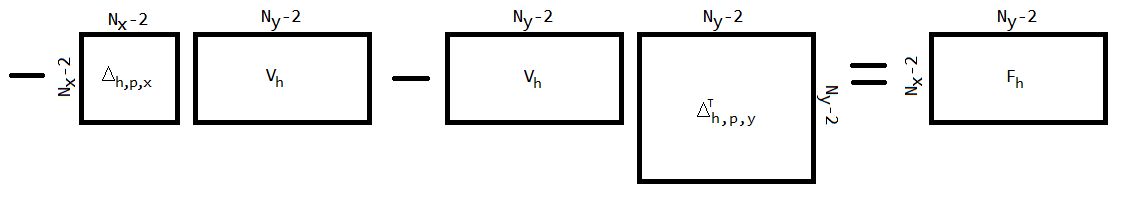
\includegraphics[width=\linewidth]{FPSExplained.png}
	\caption{Дискретното уравнение на Лаплас \rf{PsnDiscret} в матричен вид}
	\label{fig:FPSexplained}
\end{figure}
\FloatBarrier
Този тип запис на задачата \rf{PoissonEq} е разгледан от Том Личи в \cite{ref34}, където областта е квадратна $L_x = L_y$ и са използвани централни крайни разлики от втори ред $p=2$ с нулево гранично условие в $\partial \Omega_h$. При $p=2$ операторите $\Delta_{h,2,x}$ и $\Delta_{h,2,y}$ са симетрични, което допълнително улеснява търсенето на решение на поставената задача. Настоящата глава се явява разширение на горепосочения труд при произволна правоъгълна област с размери $2L_x \times 2L_y$ и несиметрични крайни разлики по границата на областта, където се прилага нулево гранично условие. Т.е. в общия случай матриците $\Delta_{h,p,x}$ и $\Delta_{h,p,y}$ не са симетрични.

\iffalse
Нека за матриците $(\Delta_{h,p,x})^T$ и $(\Delta_{h,p,y})^T$ имаме следните собствени стойности $\lambda_{x,i}$, $\lambda_{y,j}$ и собствени вектори $s_{x,i}$, $s_{y,j}$:
\begin{align}
S_x:=[s_{x,1},..,s_{x,N_x-2}],\\
D_x:= diag(\lambda_{x,1},..,\lambda_{x,N_x-2}),\\
S_y:=[s_{y,1},..,s_{y,N_y-2}],\\
D_y:= diag(\lambda_{x,1},..,\lambda_{x,N_y-2}).
\end{align}
Така се получава, че
\begin{align}\label{eigIdentity}
(\Delta_{h,p,x})^T  S_x = S_x  D_x\nonumber\\
(\Delta_{h,p,y})^T   S_y = S_y  D_y,
\end{align}
където $S_x, S_y$ се явяват матриците със собствени вектори и $D_x, D_y$ са диагоналните матрици със собствени стойности съответно на $(\Delta_{h,p,x})^T, (\Delta_{h,p,y})^T$. Последните са пресметнати, използвайки специализиран софтуер и библиотеки за работа с големи матрици. Ако положим
\be\label{subst}
X_h := ( S_x^T  V_h  S_y ) \quad \text{с размери} (N_x-2)\times(N_y-2),
\ee
и заместим в \rf{PsnDiscret}, се получава:
\be
-\Delta_{h,p,x}  (S_x^T)^{-1} X_h  S_y^{-1}  -(S_x^T)^{-1} X_h  S_y^{-1}  (\Delta_{h,p,y})^T = F_h.
\ee
След извършване на серия от прости математически операции, последният израз добива вида:
\be\label{fpp2}
- D_x  X_h -X_h  D_y = S_x^T  F_h  S_y.
\ee
Уравнение \rf{fpp2} е еквивалентно на
\be\label{fpp3}
-X_{i,j} \lambda_{x,i} - \lambda_{y,j} X_{i,j} = b_{i,j}.
\ee
разписано по компоненти и така се получава, че
\be\label{fpp4}
X_{i,j} = - b_{i,j}/(\lambda_{x,i} + \lambda_{y,j} ),
\ee
където $X_h = (X_{i,j})$ и $S_y^T  F_h   S_x = (b_{i,j})$ и това важи за всяко $(i,j)$:
$$i = 1,..,N_x-2, \quad j = 1,..,N_y-2 $$
с уточнението че $i = 0,N_x-1$, $j = 0,N_y-1$ са граничните стойности които не присъстват експлицитно в уравненията, но са взети в предвид. Имайки $X_h$ лесно може да получим $V_h$  с обратната субституция на \rf{subst}, която е 
\be\label{substInv}
V_h = (S_x^T)^{-1}  X_h  S_y^{-1}.
\ee

Изчислителната сложност при обръщането на оператора на Лаплас по метода в предходната част \ref{FPS} се разделя на две части. \textbf{ Първата част (I)} е свързана с изчисляването на собствените стойности $D_x, D_y$ и вектори $S_x, S_y$ на двете матрици $(\Delta_{h,p,x})^T$ и $(\Delta_{h,p,y})^T$. Също така се включват и пресмятанията, необходими за получаването на обратните матрици $(S_x^T)^{-1}$ и $S_y^{-1}$. Сложността на тези две процедури се оценя на $O(N_x^3+N_y^3)$ (\cite{ref260}) и съответно на $O(N_x^{2.37}+N_y^{2.37})$ (\cite{ref27}). \textbf{Втората част (II)} е свързана предимно с умножение на неразредени матрици в дясната част на \rf{fpp2} и обратната субституция \rf{substInv}, като и в двата случая произведението се формира от три матрици  с големини както следва: първата - $(N_x-2) \times (N_x-2)$, втората (средната) - $(N_x-2) \times (N_y-2)$ и третата - $(N_y-2) \times (N_y-2)$. \textbf{Това води} до изчислителна сложност от порядък
\be\label{fpsComplex}
O(N_x N_y \bar{\epsilon}),
\ee
\textbf{където $\bar{\epsilon} \in (0, max(N_x, N_y))$ (\cite{ref26, ref27})}. В случая, когато областта е квадратна, $N_x = N_y$ се получава, че $\bar{\epsilon} = 0.37 N_x$, т.е. алгоритмичната сложност е $O(N_x^{2.37})$. При метода на Тейлор изчисленията, описани в (I), се правят еднократно и получените резултати се използват в частта (II), която се прави за всеки слой по времето, т.е. (II) и \rf{fpsComplex} са с по-голяма тежест. 
\fi

\vspace{0.5cm}
\textbf{Глава 3. Формулировка и числено решение на двумерното стационарно уравнение на Бусинеск - Метод на простата итерация}

\textbf{Част 3.1} Метод на простата итерация за числено решаване на стационарното Парадигматично уравнение на Бусинеск \rf{eq45}

Тук е описана числената имплементация на метода на простата итерация за решаване на системата от две елиптични уравнения \begin{equation}\label{eq45}
\begin{split}
 &- (1 - c^2 \beta) \widehat{v}_{yy} -\widehat{v}_{xx} + \beta (1-c^2) \widehat{v} - \alpha \beta \theta \widehat{v}^2 = \widehat{w}, \\
 &- \Delta \widehat{w} =  c^2 \beta \widehat{v}_{xx},
\end{split}
\end{equation}
която е еквивалентна на задачата \rf{eq2} и $\theta$ е стойността на максимума на търсената функция $\widehat{v}$ в нулата (виж \cite{ref16}). Дефинирана е явна диференчна схема за частните диференциални уравнения:
\begin{align}\label{eq5}
\begin{split}
 &\frac {\partial \widehat{v}}{\partial t} - (1 - c^2 \beta) \widehat{v}_{yy} -\widehat{v}_{xx} + \beta (1-c^2) \widehat{v} - \alpha \beta \theta \widehat{v}^2 = \widehat{w}, \\
 &\frac {\partial \widehat{w}}{\partial t} - \Delta \widehat{w} =  c^2 \beta \widehat{v}_{xx},
\end{split}
\end{align}
чието решение се схожда към численото такова на уравненията \rf{eq45}.
Използвани са два варианта за начални стойности, с които започва първата итерация. Описано е как се променя стъпката по времето и какъв е критерият за спиране на итерационния алгоритъм. В последствие са дефинирани алгоритмичните стъпки, с които може да се възпроизведе целият итерационен процес и е изведена алгоритмичната сложност. В Таблица \ref{tab:a} е представен редът на сходимост от метода на простата итерация.

\begin{table}[ht]
\begin{small}
\centering
		\begin{tabular}{||c|l|ll|ll||}
			\hline
			\hline
      \multirow{2  }{*}{ }        & \multirow{2  }{*}{$h$}  &  	\multirow{2  }{*}{ $\Vert \bar{ E_i} \Vert_{L_2}$ }	&Ред на	& \multirow{2  }{*}{ $\Vert \bar{ E_i} \Vert_{L_\infty}$ } 		&Ред на   \\
	                                        &                                                & 							 					&  сход. 	& 								       					& сход. \\
   					\hline 
					\hline 

$\beta = 3$ 	&0.2    										&            &            &           &   \\
      c=0.45 	&0.1    & 0.014232  						&            & 0.016732 			&   \\
   $O(h^2)$     &0.05   & 0.003238  						&2.14  & 0.003997					& 2.07 \\
\hline 
$\beta = 3$   	&0.2   &            &            &             &    \\
      $c=0.45 $ &0.1   &   0.001758   &           &  0.002499  &   \\
       $O(h^4)$	&0.05  &  0.000114 & 3.95    & 0.000168  & 3.90  \\
\hline
$\beta = 3$   	&0.2   &            &        &                  &      \\
   $c=0.45$   	&0.1   &  0.005038 &           & 0.012462       &       \\
     $O(h^6)$	&0.05  &  0.000094  & 5.74  &  0.000323 & 5.27         \\
			\hline
			\hline 	
$\beta = 1$   	&0.4   &             &           &                & \\
     $c=0.9$     &0.2   &  0.043898  &             & 0.017906      &    \\
     $O(h^2)$	&0.1  & 0.009999 & 2.13       & 0.004348      & 2.04  \\
\hline 	
 $\beta = 1$   	&0.4  &            &               &               &     \\
     $c=0.9$  	&0.2   & 0.006309  &              & 0.002965      &        \\
     $O(h^4)$	&0.1  &  0.000432 &3.87        & 0.000200 &  3.89        \\
    \hline
 $\beta = 1$	&0.4   &             &        &               &        \\
   $ c=0.9$  	&0.2   &  0.000088  &        & 0.000115      &       \\
       $O(h^6)$	&0.1  &   0.000002 &5.35  & 0.000003 &   5.04       \\
	   \hline
			\hline 
		\end{tabular}
		\caption{\normalsize Ред на сходимост при метода на простата итерация с апроксимации $O(h^{2})$, $O(h^{4})$ и $O(h^{6})$ на уравнението за Тест  1 и Тест 2. Грешките на численото решение $E_i$ са пресметнати в $L_2$ и $L_\infty$ норми.}
\label{tab:a}
\end{small}
\end{table}
\FloatBarrier

\textbf{Част 3.2} Числени резултати от метода на простата итерация за решението на стационарното Парадигматично уравнение на Бусинеск

В този подраздел са направени два числени теста при параметри $\beta = 3, c=0.45$ и $\beta = 1, c=0.9$. За тези примери са показани следните резултати. Първо, резидуалът $R$ намалява от стойности близки до $1e-1$ в първата итерация до стойности под $1e-9$ на последната итерация. Второ, показано е, че четвъртите производни на решението, които са пресметнати числено, са сходящи по правилото на Рунге \rf{Runge}. Трето, получени са решения за различни стойности на параметрите $\beta$ и $c$. Това параметрично изследване потвърждава получените в \cite{ref116,ref15} резултати като например зависимостта на формата на вълната от скоростта $c$ и дисперсията $\beta$ и асимптотичното поведение на решението при $(x^2 + y^2) \rightarrow \infty$. Най-накрая, решението от последната итерация е сравнено с ``best-fit'' апроксимационните формули от \cite{ref15}, като това сравнение е все още липсващо в литературата. 
\begin{table}[ht]
\begin{small}
\centering
\begin{tabular}{|l|c|l l|l l|}
\hline
\hline 
$\beta$	& c 	& $\|v^*-v \|_{L_2 }$ & $\|v^*-v \|_{L_\infty }$  	& $D^*_{L_2}$	& $D^*_{L_\infty }$	\\
\hline 
1& 		0.1	&	1.4772e-01 		& 	8.1024e-03 				& 2.7\%			& 1.7\%		\\
\hline 
1& 		0.3 	&	1.4310e-01 		& 	8.7770e-03				& 2.7\%			& 1.9\%		\\
\hline 
1& 		0.5 	&	1.6934e-01 		& 	1.3332e-02				& 3.5\%			& 3.3\%		\\
\hline 
1& 		0.7 	&	5.8673e-01		& 	5.1122e-02				& 14.8\%		& 16.2\%	\\
\hline 
1& 		0.9	&	2.1599e+0 		& 	1.6439e-01				& 93.1\%		& 121.2\%	\\
\hline 
\hline 
\end{tabular}
\caption{Разлики между числено решение $v$ на елиптичната задача с висок ред на апроксимация $O(h^6)$ и ``best-fit'' формулите $v^*$ от \cite{ref15} при $\beta=1$ и $c=0.1, 0.3, 0.5, 0.7, 0.9$.}
\label{tab:diff-beta1}
\end{small}
\end{table}
Резултатите от него са показани на Таблица \ref{tab:diff-beta1}, където 
$D^*_{\kappa}$ дефинира процентната разлика между двете решения: $v$ на елиптичната задача с висок ред на апроксимация $O(h^6)$ и ``best-fit'' формулите $v^*$, в ${L_2 }$ и ${L_\infty}$ норми, върху цялата област $\Omega_h$:
\be\label{diffvv}
D^*_{\kappa} := 100 \times \frac{\Vert v^*-v \Vert_{\kappa} }{ \Vert v \Vert_{\kappa} }, \; \kappa=2; \; \kappa=\infty.
\ee
Това се оказва съществен елемент и повратна точка в изследването на хиперболичната задача \rf{eq1}-\rf{eq11}. \\

\textbf{Част 3.3} Ново гранично условие за двумерното елиптично уравнение \rf{eq2}
\begin{figure}[ht]
	\begin{minipage}[b]{0.85\linewidth}
		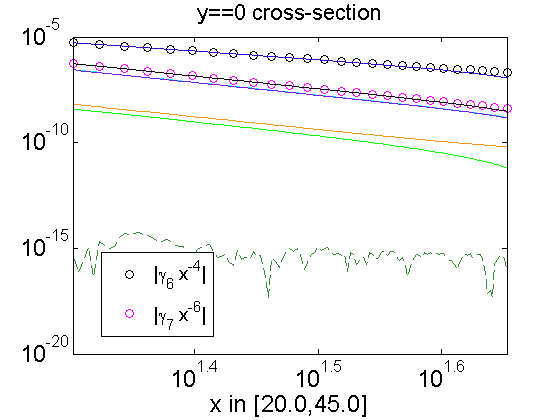
\includegraphics[width=\linewidth]{AssymptForEachTerm/c017_bt1_5/ChristovIC_AlongX_50_ZB2_bt1_c017_h020_O(h^6).png}
	\end{minipage}
	\begin{minipage}[b]{0.85\linewidth}
		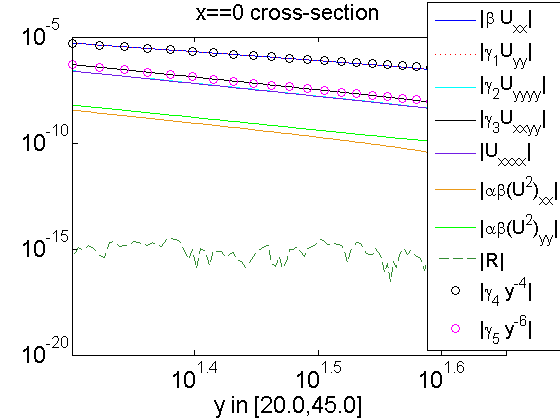
\includegraphics[width=\linewidth]{AssymptForEachTerm/c017_bt1_5/ChristovIC_AlongY_50_ZB2_bt1_c017_h020_O(h^6).png}
	\end{minipage}
	\caption{Асимптотично поведение на членовете от елиптичното уравнение, представени в абсолютна стойност и логаритмични скали по $x,y$, получено с апроксимация от шести ред и нулево гранично условие. Скоростта и дисперсионният параметър са $\boldsymbol{c=0.17}$ и $\boldsymbol{\beta = 1}$. }
	\label{fig:assympt_c017bt1}
\end{figure}
\FloatBarrier
Изведено е едно ново асимптотично гранично условие (виж \cite{bnd}) за решението на стационарното елиптично уравнение на Бусинеск \rf{eq2}. В серия от числени експерименти при $\beta=1,3,5$, $c=0.17$ и при $\beta=1$, $c=0.1, 0.5, 0.9$ е разгледана асимптотиката на всеки един от членовете за достатъчно голям радиус $r=\sqrt{x^2 + y^2} >> 0$ (виж Фигура \ref{fig:assympt_c017bt1}). Показано е, че асимптотиката на членовете с четвърти производни и нелинейните такива: 
$$- v_{xxxx}, \;  - (2-\beta c^2)v_{xxyy},  \;  - (1-\beta c^2)v_{yyyy}, \;  - \alpha \beta (v^2)_{xx}, \; - \alpha \beta (v^2)_{yy}$$
е от порядък $O(r^{-6})$, а на членовете с втори производни 
$$\beta v_{xx}, \; \beta (1-c^2) v_{yy}$$
 е от порядък $O(r^{-4})$. Използвайки тази зависимост, членовете с асимптотика $O(r^{-6})$ в елиптичното уравнение са пренебрегнати. Това води до извеждането на явната формула за гранично условие
\be
\tilde v(x, y) = \mu_v \frac{ (1-c^2) x^2 - y^2 }{ ((1-c^2) x^2 + y^2)^2 }, \quad x^2+y^2 >> 0.
\ee
Последната формула е валидирана с помощта на два числени теста. При първия експеримент разглеждаме поведението на решението по границата, когато размерите на дискретната област $\Omega_h$ нарастват - $L_x = L_y = 20, 40, 80, 160$. При вторият тест разглеждаме поведението на функцията $\widehat v$ и нейната асимптотика по $x,y$ осите.\\

\textbf{Част 3.4} Изводи

Приложен е метод на простата итерация за системата от елиптични диференциални уравнения  \rf{eq45}, изследвана с два типа начални данни:  ``best-fit'' апроксимационните формули от \cite{ref15} и числено решение на задачата \rf{eq45} при $c=0$, известно като ``Основно състояние'' (Ground state) и описано в \cite{ref1c0, ref2c0}. С първия тип начални данни решението схожда между $5-10\%$ по-бързо за случаите, които са разгледани в тази работа. Добавен е адаптивен метод за определяне на стъпката по фиктивното време, което ускорява процеса на схождане. Разписани са ясни критерии за спиране на итерационната процедура. 

Таблица \ref{tab:a} 
показва, че скоростта на сходимост, върху три вложени мрежи по правилото на Рунге \rf{Runge}, отговаря на реда на избраната апроксимация на вторите производни. При $p=6$ резултатите за сходимостта в $L_2$ и $L_\infty$ норми са по-малки от очакваното, но са по-големи от 5, което не може да се постигне с крайни разлики от четвърти ред. Диференчната схема, която отговаря на уравнение \rf{eq5}, е удовлетворена с голяма прецизност, както от апроксимации на вторите производни с до шести ред, така и от ниския праг $\epsilon \le 1\times10^{-9}$ заложен в стоп критерия.  Дискретните производни $v_{\widehat{xxxx}}$, $v_{\widehat{xxyy}}$ и  $v_{\widehat{yyyy}}$ са ограничени и сходящи. 

Представен е обширен анализ между разликите в численото решение в началния и крайния моменти от време (виж Таблица \ref{tab:diff-beta1}). 

В серия от числени експерименти се показва, че асимптотиката на членовете с производни от четвърти ред и нелинейните такива с производни от втори ред
\be\label{vtoriRed}
- v_{xxxx}, \;  - (2-\beta c^2)v_{xxyy},  \;  - (1-\beta c^2)v_{yyyy}, \;  - \alpha \beta (v^2)_{xx}, \; - \alpha \beta (v^2)_{yy}
\ee
e $O(r^{-6})$, а за останалите от втори ред
$$
\beta v_{xx}, \; \beta (1-c^2) v_{yy}
$$
асимптотиката е $O(r^{-4})$. 

Представеният анализ дава основание да пренебрегнем членовете описани в \rf{vtoriRed} и да търсим точно решение на останалата част, чрез метода на разделяне на променливите. Така извеждаме следното гранично условие
\be
\tilde v(x, y) = \mu_v \frac{ (1-c^2) x^2 - y^2 }{ ((1-c^2) x^2 + y^2)^2 },
\ee
което позволява използване на симетрични крайни разлики и по границата на областта.
\newpage
\textbf{Глава 4 Формулировка и числено решение на двумерното Парадигматично уравнение на Бусинеск} 

За удобство правим следната смяна на променливите (виж \cite{ref25}):

\be\label{vcHyp}
x = \sqrt{\beta_1} \bar{x}, \quad y = \sqrt{\beta_1} \bar{y}, \quad t = \sqrt{\beta_1} \bar{t} ,
\ee
която променя основното уравнение \rf{eq1} в
\be\label{problemVC}
 \beta (E_1-\Delta) \frac{\partial^2}{\partial t^2}u= 
(I-\Delta)\Delta u +\Delta( (\beta - 1 )u - \alpha \beta u^2 )
\ee
където $\beta = \beta_1/\beta_2$, а $E_1$ е тъждествения оператор.За улеснение навсякъде по-надолу в текста ще се използват отново старите означения $x,y,t$ вместо ${\overline x},{\overline y},{\overline t}$. \\

\textbf{Част 4.1} Дискретен закон за запазване на енергията на Консервативната схема

За Консервативната схема е изведена енергията:
\begin{align}\label{en_norm}
E_h(&v^{(k)})=\left< \left( \beta (E_1+A_h^{-1})- \frac{\tau^2}{4}( E_1+A_h ) \right)v_{t}^{(k)} ,v_{t}^{(k)} \right>+ \nonumber\\
&+\frac{1}{4}  \left<  ( E_1+A_h)(v^{(k+1)}+v^{(k)}), v^{(k+1)}+v^{(k)} \right> - \nonumber\\
&- \frac{\alpha \beta}{3} \left< ((v^{(k+1)})^3,1)+((v^{(k)})^3,1) \right> + \nonumber\\
&+\frac{\beta - 1}{2} \left< \left( (v^{(k+1)})^2+(v^{(k)})^2 \right), 1 \right>.
\end{align}
и в Теорема 1. е показано, че тя е константа величина във всеки един момент от време $t=\tau k$. В Теорема 2. е изведено условието за устойчивост
\be
\tau^2 < \frac{ 4 \beta h^2 } { 8 + h^2}, \; \beta \ge 1,
\ee 
което важи само за линейната част съответстваща на консервативното диференчно уравнение. С помощта на законите за запазване на енергията е изведена Консервативната схема за Парадигматичното уравнение на Бусинеск както е описано в \cite{ref25, ref999, ref1000}.\\
\\

\textbf{Част 4.2} Свойства на Консервативна схема

Показана е сходимостта на численото решение по правилото на Рунге \rf{Runge} върху три вложени мрежи, която варира между $1.41$ и $2.14$ за различните параметри $\beta$ и $c$ и разгледаните норми $L_2$ и $L_\infty$. Развитие във времето за дискретната енергия \rf{en_norm} е показано на Фигура \rf{EnOnly}. Скоростта ѝ на сходимост по правилото на Рунге \rf{Runge} варира между $2.00$ и $2.52$ за различните параметри $\beta$ и $c$ и разгледаните норми $L_2$ и $L_\infty$.
\begin{figure}[ht]
	\begin{minipage}[b]{0.49\linewidth}
		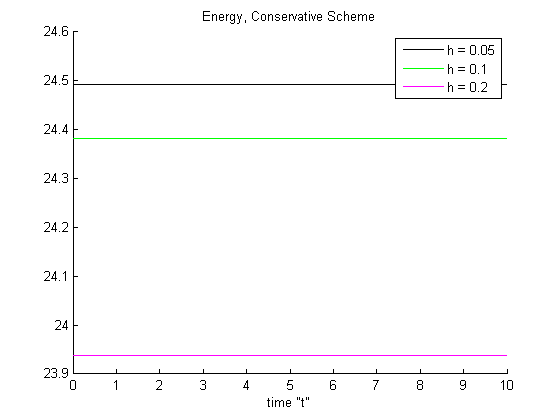
\includegraphics[width=\linewidth]{../amitans/figures/Energy_EnergySave_bt3_c045_x3O.png}	
	\end{minipage}
	\begin{minipage}[b]{0.49\linewidth}
		 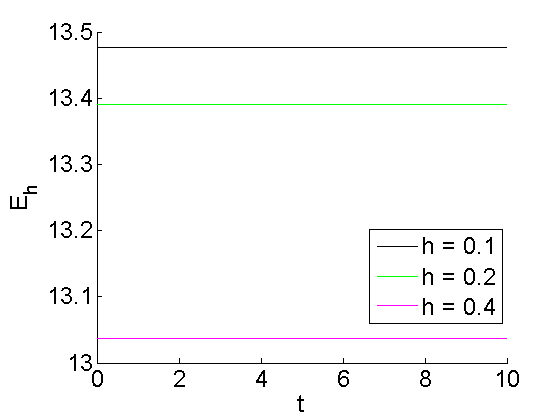
\includegraphics[width=\linewidth]{../amitans/figures/Energy_EnergySave_bt1_c090_x3O.png}
	\end{minipage}
\caption{Дискретната енергия на решението от Консервативната схема при Тест 1 (ляво) и Тест 2 (дясно) с апроксимационна грешка $O(|h|^2 + \tau^2)$ във времето $T_{\tau} = [0, 10]$.}
\label{EnOnly}
\end{figure}
За изчислението на члена $A_h^{-1}v_{t}^{(k)}=$ $-\Delta_{h,2}^{-1}v_{t}^{(k)}$ от \rf{en_norm} се използват бързите директни методи за обръщане на дискретния оператор на Лаплас, дефинирани в Част 2.6.\\

\textbf{Част 4.3} Метод на Тейлор и метод на правите за хиперболичната задача

Хиперболичното частно диференциално уравнение се разделя на система от $N_x \times N_y$ обикновени диференциални уравнения, както сме показали в \cite{refHyp}, където $N_x$ и $N_y$ са броят точки в мрежата $\Omega_h$, съответно по $x$ и $y$ осите:
\begin{align} \label{DiscreteEq}
\beta (E_1-\Delta_{h,p}) \frac{\partial^2 }{\partial t^2}u_{i, j}(t)= \nonumber \\
 (E_1 - \Delta_{h,p})\Delta_{h,p} u_{i, j}(t) + \Delta_{h,p} ( -\beta f( u_{i, j}(t) ) + (\beta-1) u_{i, j}(t) ), \nonumber \\
i = 0,\cdots, N_x-1, \: j = 0 ,\cdots , N_y-1.
\end{align}
 Всяко от уравненията е решено числено с явния метод на Тейлор спрямо времевата променлива $t$:
\begin{align} \label{TSe}
u_{i, j}(t+\tau) = u_{i, j}(t) + \tau \frac{ \partial }{ \partial t }u_{i, j}(t)  + ... 
\frac{ \tau^p }{ p! } \frac{ \partial^p}{ \partial t^p }u_{i, j}(t) + O(\tau^{p+1})
\end{align}
при $p \ge 2$. За обръщането на оператора $(E_1-\Delta_{h,p})$ използваме така наречените ``Fast Poisson Solvers'', които са описани в Част 2.6. Редът на апроксимация по времето зависи от броя на членовете $p+1$, които участват в реда на Тейлор. По този начин редът на апроксимация по времето и пространството е еднакъв, и зависи от избора на $p$.
 Производните, в реда на Тейлор, са намерени посредством диференциране по времето на уравнение \rf{DiscreteEq}.\\

\textbf{Част 4.4} Числени резултати от Консервативната схема и метода на Тейлор

В тази част са представени резултати от имплементираните методи за хиперболичната задача.
\begin{table}[ht]
\begin{small}
\centering
\small
		\begin{tabular}{||c|l|ll|ll||}
			\hline
			\hline


      \multirow{2  }{*}{$p=2,4,6$}        & \multirow{2  }{*}{$h$, $\tau$}  &	\multirow{2  }{*}{  $\Vert \bar E_i \Vert_{L_2} $ } 	&Ред на & \multirow{2  }{*}{  $\Vert \bar E_i \Vert_{L_\infty}$ }	&Ред на   \\
	                                        &                                                &    										&  сход. & 										& сход. \\
\hline 
\hline 
  $\beta=3$               &0.2, 0.1      &              	&           &                	&      \\
   c=0.45                   &0.1, 0.05    &0.968044  	&           &1.034208   &       \\
 $O(h^2 + \tau^ 2)$ 	&0.05, 0.025	& 0.340955 	& 1.51    &0.351518  	&  1.56      \\
\hline 
  $\beta=3$               &0.2, 0.1      &              	&          	&                 &      \\
   c=0.45                   &0.1, 0.05    &0.191389 	&          	&0.194056   	&       \\
$O(h^4+ \tau^4)$	&0.05, 0.025	&0.013036 	& 3.88   	&0.013664   	& 3.83       \\
\hline 
  $\beta=3$               &0.2, 0.01    &                	&          	&                 &      \\
     c=0.45                 &0.1, 0.05    &0.032671 	&          	& 0.033625  	&       \\
  $O(h^6+ \tau^6)$ 	&0.05, 0.025	&0.000599 	&5.78    	& 0.000635  	& 5.73       \\
\hline
\hline 
       $\beta=1$        	&0.4, 0.2      &             	&            &           &   \\
           c=0.9    		&0.2, 0.1      &  0.148014 	&            &0.058905 &   \\
  $O(h^2+ \tau^2)$  	&0.1, 0.05   	& 0.030690  	&2.27  	 &0.014185   & 2.05 \\
\hline
      $\beta=1$           &0.4, 0.2    	&            	&               &             &    \\
       c=0.9                 &0.2, 0.1     & 0.028869   &        &  0.013791   &   \\
 $O(h^4+ \tau^4)$ 	&0.1, 0.05   	&0.001860 	& 3.96  & 0.000996  & 3.80  \\
\hline
  $\beta=1$     		&0.4, 0.2   	&            	&          	&                  &      \\
      c=0.9                  &0.2, 0.1   	&0.006732 	&            & 0.003334      &       \\
 $O(h^6+ \tau^6)$ 	&0.1, 0.05 	& 0.000249 	& 4.75 	& 0.000068  & 5.61        \\
\hline
\hline 
		\end{tabular}
		\caption{Скорост на сходимост на численото решение при метода на Тейлор с нулево гранично условие и грешки от апроксимацията $O(|h|^{2} + \tau^2 )$, $O(|h|^{4} + \tau^4 )$ и $O(|h|^{6} + \tau^6 )$. Грешките $\bar E_i$ са измерени в $L_2$ и $L_\infty$ норми.}
\label{tableA}
\end{small}
\end{table}
Редът на сходимост на дискретните решение и енергия, получени от метода на Тейлор, по правилото на Рунге \rf{Runge} са показани съответно на Таблици \ref{tableA} и \ref{tableB}. Редът на сходимост отговаря на приложения ред на апроксимация. Само при Тест 2 и $O(|h|^6 + \tau^6)$, сходимостта при енергията е по-ниска от очакваното. Този резултат е поради високия градиент на решението, близо до границата и по-ниската сходимост, получена още при началното условие от решаване на елиптичната задача (виж последният ред в Таблица \ref{tab:a}). 
\begin{table}[ht]
\begin{small}
\centering
\small
		\begin{tabular}{||c|l|ll|ll||}
			\hline
			\hline
      \multirow{2  }{*}{FDS}        & \multirow{2  }{*}{$h$, $\tau$}  &  	\multirow{2  }{*}{ $\Vert \bar{\bar{ E_i}} \Vert_{L_2}$ }	&Ред на	& \multirow{2  }{*}{ $\Vert \bar{\bar{ E_i}} \Vert_{L_\infty}$ } 		&Ред на   \\
	                                        &                                                & 							 					&  сход. 	& 								       					& сход. \\
   			\hline 
					\hline 
  $\beta=3$             	&0.2, 0.1         	&              	&          	&                     &      \\
   c=0.45                 	&0.1, 0.05         	&0.379690  	&          	&0.446557 		&       \\
 $O(h^2 + \tau^ 2)$ 	&0.05, 0.025  	& 0.075257 	& 2.33  	& 0.111797     	& 2.00      \\
\hline 
  $\beta=3$               &0.2, 0.01       	&                	&          	&                     	&      \\
   c=0.45                   &0.1, 0.005      	&0.044788 	&         	&0.082344   		&       \\
 $O(h^4+ \tau^4)$ &0.05, 0.025  		&0.002459 	&4.18    	&0.003562   		&4.53      \\
\hline 
  $\beta=3$               &0.2, 0.01       	&                	&          	&                 	&            \\
     c=0.45                 &0.1, 0.05        	&0.063681 	&          	&  0.133517  	&           \\
 $O(h^6+ \tau^6)$ &0.05, 0.025 		&0.001086 	& 5.87   	&  0.002041		&6.03   \\
\hline
\hline 
       $\beta=1$       	&0.4, 0.2     		&             	&           &           		&   \\
                  c=0.9    	&0.2, 0.1     		& 0.404499 	&           &0.348428 		&   \\
$O(h^2+ \tau^2)$ 	&0.1, 0.05   		& 0.081033  	&2.32  	&0.087663  		& 2.00 \\
\hline
      $\beta=1$           &0.4, 0.2    		&            	&        	&             		&    \\
       c=0.9                	&0.2, 0.1     		& 0.064165  	&        	&  0.056574   	&   \\
$O(h^4+ \tau^4)$ 	&0.1, 0.05   		&0.005141 	& 3.64  	& 0.005173  		& 3.45  \\
\hline
  $\beta=1$     	 	&0.4, 0.2   		&            	&         	&                  	&      \\
      c=0.9                 	&0.2, 0.1   		&0.037448	&         	& 0.054236      	&       \\
   $O(h^6+ \tau^6)$ &0.1, 0.05  		& 0.003098 	& 3.60 	& 0.003293  		& 4.04        \\
\hline
\hline 
		\end{tabular}
		\caption{Скорост на сходимост на дискретната Енергия при метода на Тейлор с нулево гранично условие и грешки от апроксимацията $O(|h|^{2} + \tau^2 )$, $O(|h|^{4} + \tau^4 )$ и $O(|h|^{6} + \tau^6 )$. Грешките $\bar{\bar E_i}$ са измерени в $L_2$ и $L_\infty$ норми.}
\label{tableB}
\end{small}
\end{table}
\FloatBarrier
Дискретните енергия и маса се пресмятат на всяка стъпка по времето и са вектори с дължина $N_t - 1$. При Консервативната схема енергията е получена чрез формула \rf{en_norm} $(O(h^{2}))$, а при метода на Тейлор с правилата на трапците, Симпсън и Буул, съответно с грешка от апроксимациите $O(h^{2})$, $O(h^{4})$ и $O(h^{6})$ (виж Фигура \ref{EnTest1Test2}). 
\begin{figure}[ht]\vspace{0.2cm}
	\begin{minipage}[b]{0.51\linewidth}
		%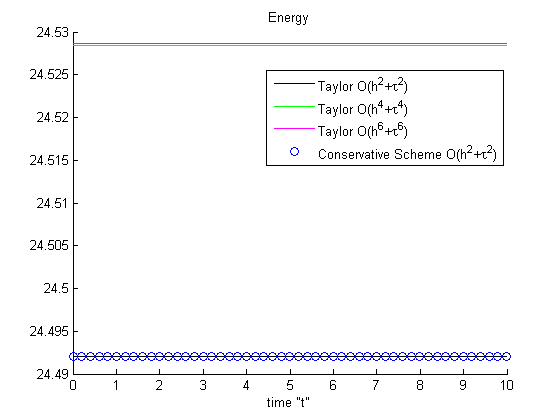
\includegraphics[width=\linewidth]{../amitans/figures/Energy_bt3_c045_h005_Taylor_Conservative.png}	
		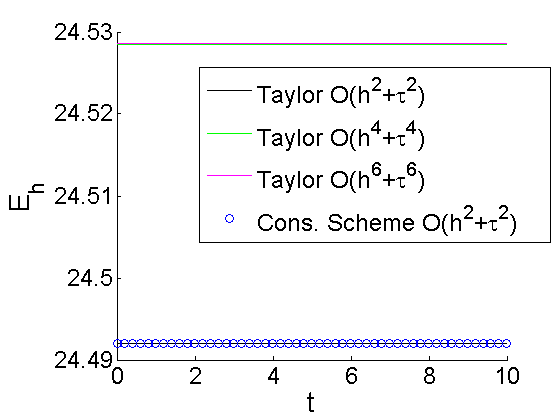
\includegraphics[width=\linewidth]{Energy/Energy_bt3_c045_h005_Taylor_Conservative.png}	
	\end{minipage}
	\begin{minipage}[b]{0.51\linewidth}
		%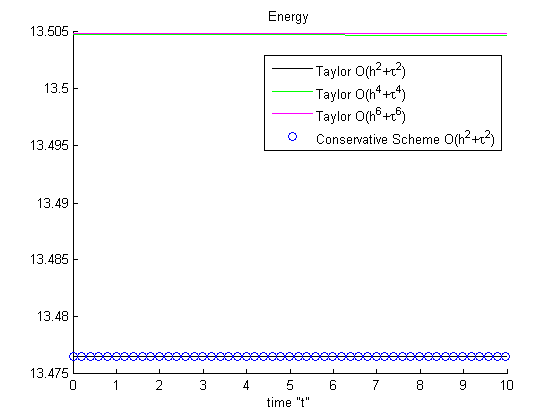
\includegraphics[width=\linewidth]{../amitans/figures/Energy_bt1_c090_h010_Taylor_Conservative.png}		
		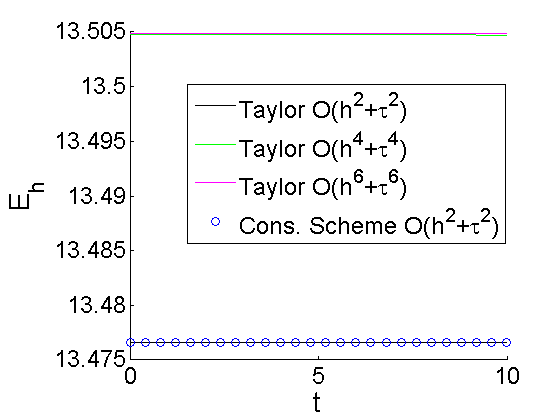
\includegraphics[width=\linewidth]{Energy/Energy_bt1_c090_h010_Taylor_Conservative.png}				
	\end{minipage}
\caption{Дискретнa eнергия на решението като функция на времето до $T=10$ при Тест 1 (ляво) и Тест 2 (дясно).}
\label{EnTest1Test2}
\FloatBarrier
\end{figure}
Направени са допълнителни изчисления върху области с по-големи размери и по-голяма стъпка $h=0.5$, за да се обясни нарастването при масата, като резултатите от изследванията са показани на Фигура \rf{Test1_2Mass}.
\begin{figure}[ht]\vspace{0.2cm}
	\begin{minipage}[b]{0.51\linewidth}
		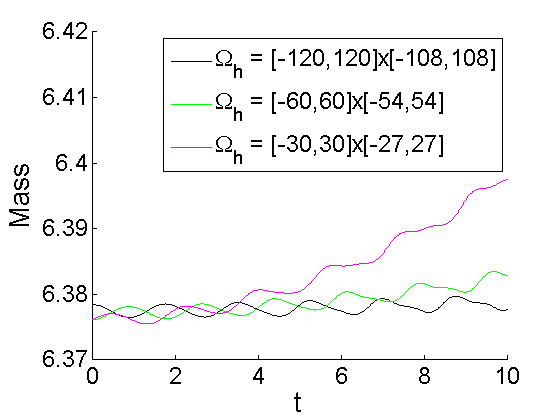
\includegraphics[width=\linewidth]{Mass/MassTaylor_120_60_30_ZB1_bt3_c045_h020_O(h^6).png}
	\end{minipage}	
	\begin{minipage}[b]{0.51\linewidth}
		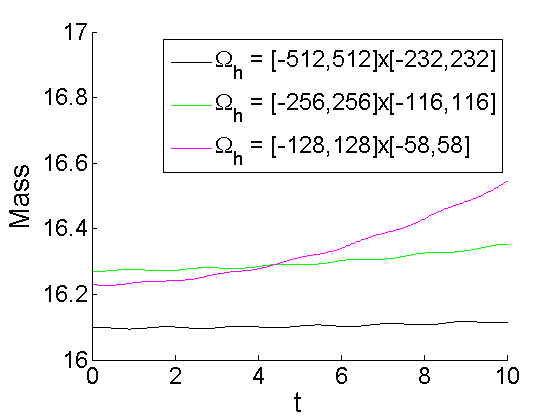
\includegraphics[width=\linewidth]{Mass/MassTaylor_512_256_128_ZB1_bt1_c090_h040_O(h^6).png}
		
	\end{minipage}
\caption{Масата от решението от метода Тейлор с $O(|h|^6 + \tau^6)$ апроксимация като функция на времето до $T=10$ върху три различни по големина области. Левият панел е при $\beta =  3$, $c = 0.45$, а десният панел е при $\beta =  1$, $c = 0.9$.}
\label{Test1_2Mass}
\end{figure}
\FloatBarrier
Направени са сравнения между решенията, получени от двата различни подхода: Консервативната схема и метода на Тейлор, като получените резултати, измерени в $L_2$ и $L_\infty$ норми, са близки. Представен е анализ на зависимостта на формата и максимума от реда на апроксимация и големината на дискретните стъпки по пространството и времето - $h, \tau$. 
\begin{table}[ht]
\begin{small}
\centering
\small
		\begin{tabular}{||c|l|l|l||}
			\hline
			\hline
        $p$       & $h$, $\tau$  & $||u^{(0)} - u^{(N_t)}||_{L_2}$  & $||u^{(0)} - u^{(N_t)}||_{L_\infty}$   \\
   		\hline 
			\hline
  $\beta=3$                &0.2, 0.001            & 1.494351 & 1.533173    \\
   c=0.45                     &0.1, 0.0005          & 0.466991 & 0.484011       \\
     $O(h^2 + \tau^ 2)$ &0.05, 0.00025   & 0.127641 & 0.132504      \\
			\hline 
  $\beta=3$               &0.2, 0.02       &0.220560 & 0.230486       \\
   c=0.45                    &0.1, 0.01      &0.013762 & 0.014391        \\
     $O(h^4+ \tau^4)$ &0.05, 0.005&0.000877 & 0.000917         \\
			\hline 
  $\beta=3$               &0.2, 0.02        &  0.035965 & 0.038039        \\
     c=0.45                 &0.1, 0.01        &0.000600 & 0.000633       \\
     $O(h^6+ \tau^6)$ &0.05, 0.005 &0.000010 & 0.000010          \\
	   \hline
			\hline 
       $\beta=1$       &0.4, 0.002        & 0.244208 & 0.103833 \\
                  c=0.9    &0.2, 0.001       &  0.057175 & 0.026919  \\
  $O(h^2+ \tau^2)$ &0.1, 0.0005   & 0.013938 & 0.006622  \\
			\hline
      $\beta=1$               &0.4, 0.04     &0.028546 & 0.012203 \\
       c=0.9                     &0.2, 0.02     & 0.001757 & 0.000958     \\
       $O(h^4+ \tau^4)$ &0.1, 0.01   & 0.000112 & 0.000061   \\
    \hline
  $\beta=1$                  &0.4, 0.04   &0.006415 & 0.002792  \\
      c=0.9                    &0.2, 0.02   &0.000112 & 0.000065     \\
     $O(h^6+ \tau^6)$ &0.1, 0.01 & 0.000002 & 0.000001         \\
	   \hline
			\hline 
		\end{tabular}
		\caption{Разликата $||u^{(0)} - u^{(N_t)}||_\kappa$ в $L_2$ и $L_\infty$ норми между решенията в началния $t=0$ и крайния $t=10$ моменти от време. За резултатите от таблицата е използван единствено методът на Тейлор.}
\label{tableG}
\end{small}
\end{table}
\FloatBarrier
Таблица \ref{tableG} показва, че с намаляване на стъпките по пространството $h$ и времето $\tau$, разликата в профила на вълната между началния и крайния момент също намалява. Най-накрая е разгледан случай при по-голям времеви интервал $T=30$, за който отново са описани поведението на формата и максимума.\\

\textbf{Част 4.5} Числен тест за хиперболичната задача при параметри $\beta = 3$ и $c=0.3$

Настоящата част разглежда един добре познат в литературата случай за хиперболичната задача (виж \cite{ref21, ref20, ref23, ref22} ), при който за начално условие в споменатите трудове винаги са използвани ``best-fit'' апроксимационните формули от \cite{ref15}. В настоящата работа при $t=0$ ще бъде използвано решението от стационарното уравнение на Бусинеск (еквивалентно на системата \rf{eq45}) с апроксимации от висок ред и  ``Симетрично гранично условие по абцисата и ординатата при елиптичната задача'', както е дефинирано в Част 2.3. Големината на областта $\omega_h$ е $L_x = L_y = 50$, $\alpha = 1$, а използваните крайни разлики са с четвърти и шести ред на апроксимация (при $p=4, 6$). Поради симетрията на решението по абцисата и ординатата е лесно да се построи началната функция в цялата област $\Omega_h$. При хиперболичната задача (разгледана в $\Omega_h$) е използван метод на Тейлор, отново с апроксимационни формули от четвърти и шести ред. Представен е анализ на зависимостта на формата и максимума от реда на апроксимация и големината на дискретните стъпки по пространството и времето - $h, \tau$ - за метода на Тейлор (виж Фигура \ref{MultiMaximum} и Таблица \ref{tableK}). 
\begin{figure}
	\centering
	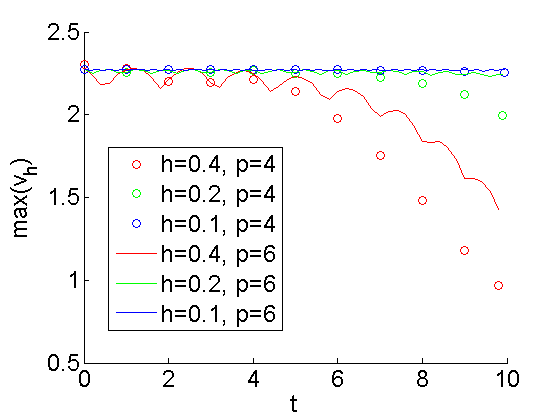
\includegraphics[width=0.70\linewidth]{Maximum_TaylorZeroBnd_50x50_bt3_c030.png}
\caption{Развитие на максимума на решението в интервала $[0, 10]$ при $\beta = 3$, $c=0.3$. За резултатите от графиката е използван метода на Тейлор с четвърти и шести порядък на апроксимация и дискретните стъпки $h=0.4, 0.2, 0.1, \tau = h/2$.}
\label{MultiMaximum}
\end{figure}
\FloatBarrier
\begin{table}[ht]
\begin{small}
\centering
\small
		\begin{tabular}{||c|l|l|l||}
			\hline
			\hline
  $p=4,6$   &  $h, \tau$ &  $||u^{(0)} - u^{(N_t)}||_{L_2}$  & $||u^{(0)} - u^{(N_t)}||_{L_\infty}$   \\
   		      \hline 
			\hline
           				& $0.4, 0.2$   &  3.020072 & 2.571611     \\
			\hline 
  $O(|h|^4+\tau^4)$ & $0.2, 0.1$   & 0.365473 & 0.371433      \\
			\hline 
           				& $0.1, 0.05$ & 0.025631 & 0.026517      \\
	   \hline
          \hline
           				& $0.4, 0.2$   & 1.939208 & 1.673675      \\
			\hline
  $O(|h|^6+\tau^6)$ & $0.2, 0.1$   & 0.037638 & 0.038985      \\
    \hline
           				& $0.1, 0.05$  & 0.000655 & 0.000679       \\
	   \hline
		\hline 
		\end{tabular}
		\caption{Разлика $||u^{(0)} - u^{(N_t)}||_\kappa$ в $L_2$ и $L_\infty$ норми между числените решения в началото при $t=0$ и в края при $t=10$. За резултатите в таблицата е използван методът на Тейлор с четвърти и шести порядък на апроксимация. }
\label{tableK}
\end{small}
\end{table}
\FloatBarrier
\begin{figure}
	\centering
	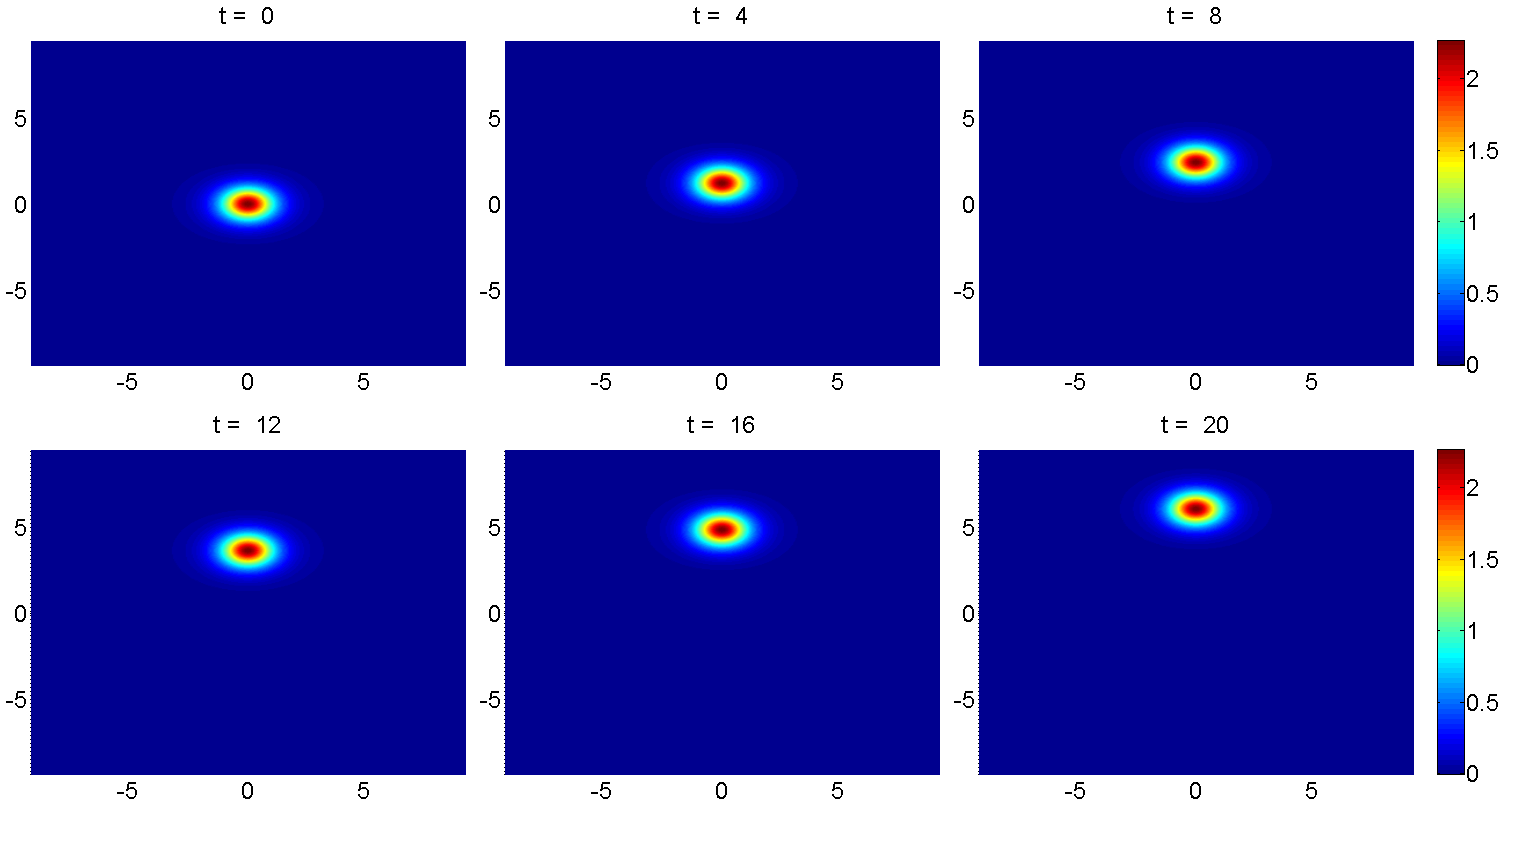
\includegraphics[width=\linewidth]{SolutionView/TaylorZeroBnd_50_ZB2_bt3_c030_h005_TAll_O(h^6).png}
\caption{Развитие на формата на численото решение при $\beta = 3$, $c=0.3$. Използван е метод на Тейлор с апроксимация от шести ред и следните дискретни стъпки: $h=0.05, \tau = 0.025$. По вертикалата е $y$ оста, а по хоризонталата $x$ оста.}
\label{solShape3}
\end{figure}
\FloatBarrier
Разгледан е случай при по-голям времеви интервал $T=30$, за който отново са описани поведението на формата и максимума. Развитието на вълната до време $t=20$ не търпи видими структурни промени, както е показано на Фигура \ref{solShape3}.\\

\textbf{Част 4.6} Изводи

Показали сме как се извежда дискретната енергия \rf{en_norm} за Парадигматичното уравнение на Бусинеск \rf{problemVC} след смяната на променливите \rf{vcHyp}, 
базирайки се на статиите \cite{ref25, ref999, ref1000}. 
Имплементирана е консервативна схема за \rf{problemVC}, с втори ред на апроксимация, която запазва дискретната енергия \rf{en_norm} безусловно. 

Разработен е метод на Тейлор в комбинация с метод на правите за \rf{problemVC} с втори, четвърти и шести ред на апроксимация на вторите производни по пространството и времето. 
Скоростта на сходимост е измерена по правилото на Рунге \rf{Runge}, върху три вложени мрежи, понеже не е известно аналитично решение. Резултатите отговарят на приложената апроксимация
с леки отклонения (виж Таблица \ref{tableA}). 

Този алгоритъм не запазва безусловно енергията, затова тя заедно с масата и формата на решението (при $O(|h|^2 + \tau^2)$) са сравнени с тези, получени при Консервативната схема.
Резултатите от двата метода са качествено и количествено много близки. 
От числените резултати се забелязва тенденцията, че разликата между двата класа от решения намалява, 
когато стъпките $h$ и $\tau$ се свиват. 

За поведението на масата е показано, че измененията ѝ намаляват, когато задачата се пресмята в по-големи области $\Omega_h$ 
(виж Фигура \ref{Test1_2Mass}).
Таблица \ref{tableG} показва, че с намаляване на стъпките по пространството $h$ и времето $\tau$, разликата в профила на вълната между началния и крайния момент намалява. 
В допълнение се вижда, че формата на вълната се запазва по-добре, когато степента на апроксимация на диференциалните оператори е по-висока. 
Последните разсъждения затвърждават очакването, че разликата във формата на численото решение между началния и крайния моменти $||u^{(0)} - u^{(N_t)}||_\kappa$, за произволно фиксирано време $T$, клони към нула, когато $h$ и $\tau$ са много малки.

Показано е, че максимумът и формата на решението се запазват, с пренебрежимо малки отклонения, за по-голям времеви интервал $[0, 30]$. 

Разгледан е един добре познат в литературата случай за хиперболичната задача \rf{eq1} (виж \cite{ref21, ref20, ref23, ref22} ), 
при който за начално условие в споменатите трудове винаги са използвани ``best-fit'' апроксимационните формули от \cite{ref15}. 
В дисертацията при $t=0$ е използвано численото решение на елиптичната задача \rf{eq45} с четвърти и шести ред на апроксимация.
Направените числени примери показват, че с намаляване на стъпката и 
увеличаване апроксимацията на метода, максимумът и формата се запазват по-добре (виж Фигура \ref{MultiMaximum}). Освен това вълната се съхранява по-дълго, до време $t=20$ ($t_{orig}=34.64$ в оригиналните
променливи преди смяната \rf{vcHyp}).

\section{Заключение}

За решение на стационарното уравнение на Бусинеск са използвани диференчни схеми с втори, четвърти и шести ред на апроксимация на вторите производни заедно с метода на простата итерация. В Таблица \ref{tab:a} е показана скоростта на сходимост по правилото на Рунге върху три вложени мрежи, която в повечето случаи отговаря на използвания ред на апроксимация. Полученото числено решение има сходно поведение с това, описано в \cite{ref117,ref116} от гледна точка на формата и зависимостта ѝ от скоростта $c$ и дисперсионния параметър $\beta$. Получените резултати се използват за начално условие в ПУБ.

Изведено е ново асимптотично гранично условие за елиптичната задача, след като са изследвани асимптотиките на всички членове поотделно в стационарното елиптично уравнение на Бусинеск. Получената явна формула е валидирана в серия от числени експерименти при различни размери на областта $L_x=L_y=20,40,80,160$. Показано е, че численото решение се апроксимира по-добре, когато $L_x$ и $L_y$ са по-големи. Направени са изчисления с нулево гранично условие и резултатите са сравнени с новото такова, където се вижда, че $L_2$ нормата от разликата намалява два пъти, а $L_\infty$ нормата - четири пъти, при двойно увеличение на областта.

За хиперболичната задача са използвани два различни подхода - Консервативната схема и комбинацията от метод на Тейлор и метод на правите с втори, четвърти и шести ред на апроксимация, който се прилага за пръв път за ПУБ. Числените решения, заедно с неговите свойства като маса, енергия и форма, получени с метода на Тейлор и Консервативната схема, са сравнени при $O(|h|^2 + \tau^2)$ и е показано, че са доста близки. Една от целите на работата е да покаже, че методът на Тейлор, приложен към уравнението \rf{problemVC}, също води до достатъчно добри резултати, а също така може да се приложи с по-висок ред на апроксимация, което води и до по-фино решение. Числената енергия е запазена и в двата случая. При масата е показано, че се запазва по-добре върху по големи области. 

Формата и максимумът на вълната се запазват за по-дълго време до $T=34.64$ в оригиналните променливи, когато се изполват апроксимации от по-висок шести ред и начално условие получено числено чрез решение на стационарното уравнение на Бусинеск. В допълнение, формата на решението се запазва по-добре спрямо получените резултати в \cite{ref21, ref20, ref23, ref22, ref24} за дадено фиксирано време $T$ (виж Таблица \ref{tableG} и Таблица \ref{tableK}) с намаляване на дискретните съпки по времето и пространството $h, \tau$ и увеличаване реда на апроксимация на метода.

Числените алгоритми за решенията на стационарното и Парадигматичното уравнения на Бусинеск могат да бъдат намерени и клонирани от следното интернет хранилище (repository):\\
https://github.com/CloakMe/Boussinesq.git

\newpage
\section{Научни приноси}

Основните научни приноси на дисертацията са:
\begin{itemize}
  \item Разработили сме числени методи с четвърти и шести ред на апроксимация за стационарното и  Парадигматичното уравнения на Бусинеск;
  \item Изследвали сме подробно асимптотиката на всеки един от членовете в елиптичното уравнение и сме изведели ново асимптотично гранично условие; 
  \item Показали сме, че началното условие, получено чрез итерационен метод с висок ред на апроксимация за решаване на стационарното уравнение, превъзхожда ``best-fit'' апроксимационните формули, когато се изследва солитонният характер на вълната в ПУБ, защото нейните форма и максимум се запазват за по-дълъг период от време; 
  \item Числените експерименти изтъкват, че тези две свойства на решението се запазват по-добре, когато се използват по-ситни дискретни стъпки и по-висок ред на апроксимация за фиксиран интервал от време $T$. 
\end{itemize}

\section{Декларация}
Декларирам, че представената дисертация на тема: ``Числено изследване на двумерното уравнение на Бусинеск'' е мой труд. В нейното разработване не са ползвани разработки и чужди публикации в нарушение на авторските им права. 

Всички цитирания на източници на информация, текст и други са обозначени според стандартите.

Резултатите от дисертационното изследване са оригинални и не са взаимствани от източници, в които нямам участие.
\vspace{1cm}

Подпис: ...............

\newpage
\section{Благодарности и посвещение}

{\Large \it Искам сърдечно да благодаря на моя научен ръководител - проф. д-р Наталия Кольковска, за помощта и съветите, които ми даде. Продължителните дискусии, които водихме, оказаха съществено влияние върху работата по дисертацията.}

{\Large \it Благодаря на моето семейството и роднини за търпението и подкрепата, която ми оказваха през годините.}

{\Large \it Благодаря на колегите от секция ``Математическо моделиране и числен анализ'' за полезните съвети и насоки.}

{\Large \it Благодаря на Тодор Коларов, управител на Телеконт ЕООД и Димитър Димитров, управител на Диджитал Лайтс ЕООД, които ми позволиха да работя над този труд, чрез допълнителна платена отпуска.}

{\Large \it Благодаря на доц. д-р Иван Бажлеков, за предоставения достъп до неговия работен компютър, на който съм пускал изчисления в продължение на месеци.}

\vspace{4cm}

{\Large \it Въпреки че не познавам лично проф. Христо Христов, имах възможност да се запозная с  изследванията му върху Парадигматичното уравнение на Бусинеск. Посвещавам този труд на него. }

\newpage
\begin{thebibliography}{99}

	\bibitem{ref01} Boussinesq, J., Theorie de l'intumescence liquide, applelee onnde solitaire ou de translation, se propageant dans un canal rectangulaire, {\it Comptes Rendus de l'Academie des Sciences}, \textbf{72} (1871), 755-759.

	\bibitem{ref02} Boussinesq, J., Theorie des ondes et des remous qui se propagent le long d'un canal rectangulaire horizontal, en communiquant au liquide contenu dans ce canal des vitesses sensiblement pareilles de la surface au fond.  {\it Journal de Mathematiques Pures et Appliquees}, \textbf{17} (1872), 55-108.

	\bibitem{ref1} Christov, C.I., An energy-consistent dispersive shallow-water model,  {\it Wave Motion}, \textbf{34} (2001), 161-174.

	\bibitem{ref159} Todorov, M. D., Nonlinear Waves: Theory, computer simulation, experiment, Two-dimensional Boussinesq equation. Boussinesq paradigm and soliton solutions, Morgan and Claypool Publishers, California, 2018

	\bibitem{ref15} Christov, C.I., Choudhury, J., Perturbation solution for the 2D Boussinesq equation, {\it Mech. Res. Commun.}, \textbf{38} (2011), 274-281.

	\bibitem{ref21} Chertok, A., Christov, C.I., Kurganov, A., Central-Upwind Schemes for the Boussinesq Paradigm Equations,
{\it Computational Science and High Performance Computing IV, Notes Numer. Fluid Mech.}, \textbf{113} (2011), 267-281.

	\bibitem{ref20} Christov, C.I., Kolkovska, N., Vasileva, D., On the Numerical Simulation of Un-steady Solutions for the 2D Boussinesq Paragigm Equation,
{\it In: I. Dimov, S. Dimova, N. Kolkovska (Eds.), Numerical Methods and Applications 2010},
\emph{Conference Proceedings}, \textbf{6046} (2010), 386–394.

	\bibitem{ref23} M.Dimova, D. Vasileva, Comparison of Two Numerical Approaches to Boussinesq Paradigm Equation, 
{\it Numerical Analysis and Its Applications. NAA 2012. Lecture Notes in Computer Science}, \textbf{8236}, (2013), 255-262.

	\bibitem{ref22} Kolkovska N., Angelow K., A Multicomponent Alternating Direction Method for Numerical Solving of Boussinesq Paradigm Equation,
In: {\it  I. Dimov, I., Farago, I., Vulkov, L. (eds.) NAA 2012},
\emph{Conference Proceedings}, \textbf{8236} (2013), 371–378.

	\bibitem{ref25} Kolkovska N., Two families of finite difference schemes for multidimensional Boussinesq paradigm equation, In:
{\it Applications of Mathematics in Technical and Natural Sciences,  Sozopol (Bulgaria)},
\emph{AIP Conference Proceedings}, \textbf{1301} (2010), 395.

	\bibitem{ref10000} Erbay H., Erbay S., Erkip A., Instability and stability properties of traveling waves for the double dispersion equation, {\it Nonlinear Analysis}, \textbf{133} (2016), 1-14.

	\bibitem{ref1c0} Kolkovska N. Angelow K., Numerical computation of the critical energy constant for two-dimensional Boussinesq equations,
{\it Application of Mathematics in Technical and Natural Sciences, Albena (Bulgaria)},
\emph{AIP Conference Proceedings}  \textbf{1684} (2015), 080007.

	\bibitem{ref14} Christou M. , Christov C.I.,
Fourier Galerkin method for 2D solitons of Boussinesq equation,
{\it Mathematics and Computers in Simulation} \textbf{74} (2007), 82-92.

	\bibitem{ref13} Christou M. , Christov C.I.,
Galerkin spectral method for the 2D solitary waves of Boussinesq paradigm equation,
In: {\it Applications of Mathematics in Technical and Natural Sciences, Sozopol (Bulgaria)},
\emph{AIP Conference Proceedings}, \textbf{1186}, Issue 1 (2009), 217-225.

	\bibitem{ref117} J. Choudhury, C.I. Christov,
2D solitary waves of Boussinesq equation, in ISIS International Symposium on Interdisciplinary Science, Natchitoches, October 6-8, 2004, {\it APS Conference Proceedings 755}, Washington, DC, 2005, pp 85-90.

	\bibitem{ref116} C.I. Christov,
Numerical implementation of the asymptotic boundary conditions for steadily propagating 2D solitons of Boussinesq type equations,
{\it Mathematics and Computers in Simulation}, \textbf{82} (2012), 1079-1092.

	\bibitem{ref200} Vasileva, D., Kolkovska, N., Investigation of two numerical schemes for the 2D Boussinesq paradigm equation in a moving frame coordinate system, {\it In: Mathematics in industry},
\emph{Cambridge Scholars}, (2014), 289–305.

	\bibitem{ref241} M.Dimova, N. Kolkovska, Comparison of some finite difference schemes for Boussinesq Paradigm Equation, 
{\it Int. Conf. Math. Model. Comput. Phys.}, \emph{Springer}, (2011), 215-220.

	\bibitem{ref251} Kolkovska N., Four-Level Conservative Finite-Difference Schemes for Boussinesq Paradigm Equation, {\it American Institute of Physics},
\emph{AIP Conference Proceedings}, \textbf{1561} (2013), 68-74.

	\bibitem{ref252} Kolkovska N., Error Estimates of Four Level Conservative Finite Difference Schemes for Multidimensional Boussinesq  Equation,  {\it Int. Conf. Finite Differ. Methods}, \emph{Springer} (2014), 266-273.

	\bibitem{ref253} Blinkov Y., Gerdt V., Pankratov I., Kotkova E., Construction of a New Implicit Difference Scheme for 2D Boussinesq Paradigm Equation, {\it Int. Workshop Comput. Algebra Sci. Comput.}, \emph{Springer}, (2019), 152-163.

	\bibitem{ref24} Yuyu He, Hongtao Chen, Efficient algorithm and convergence analysis of conservative SAV compact difference scheme for Boussinesq Paradigm equation, 
{\it Computers and Mathematics with Applications}, \textbf{125} (2022), 34-50.

	\bibitem{ref254} Vucheva V., Kolkovska N., High Order Symplectic Finite Difference Scheme for Double Dispersion Equations, {\it AIP Publishing LLC}, \emph{AIP Conference Proceedings}, \textbf{2321}, (2021), 030037

	\bibitem{bnd} Angelow K., New Boundary Condition for the Two Dimensional Stationary Boussinesq Paradigm Equation, 
{\it International Journal of Applied Mathematics}, \textbf{32,1}, (2019), 141-154.

	\bibitem{ref999} Kolkovksa, N., Convergence of FDS for a Multidimensional Boussinesq Equation, {\it Lecture Notes in Computer Science}, \textbf{6046} (2011), 469-476.

	\bibitem{ref1000} Kolkovksa, N., Dimova, M., A new conservative finite difference scheme for Boussinesq paradigm equation, {\it Central European Journal of Mathematics}, \textbf{10} (2012), 1159-1171.

	\bibitem{refHyp} Angelow K., Comparison between two numerical methods for solution of 2D Boussinesq paradigm equation, \emph{AIP Conference Proceedings}, \textbf{2522}, (2022), 090001

	\bibitem{ref34} T. Lyche, Fast Direct Solution of a Large Linear System,
{\it Numerical Linear Algebra and Matrix Factorizations, Texts in Computational Science and Engineering}, \textbf{22}, (2020), p 237-250

	\bibitem{forn} Fornberg, B., Generation of Finite Difference Formulas on Arbitrarily Spaced Grids, 
Math. Comput., 51(1988),  699 -- 706.

	%\bibitem{boole} Zucker, Ruth, "Chapter 25.4.14: Numerical Interpolation, Differentiation, and Integration - Integration - Numerical Analysis". In Abramowitz, Milton; Stegun, Irene Ann (eds.). Handbook of Mathematical Functions with Formulas, Graphs, and Mathematical Tables. 
{\it Applied Mathematics Series} \textbf{55}  (1983), ISBN 978-0-486-61272-0.

	%\bibitem{ref260} G. H. Golub and C. F. Van Loan, Matrix Computations, 3/e, Johns Hopkins University, Press, Baltimore, 1996.

	%\bibitem{ref27} Coppersmith Don, Winograd Shmuel., Matrix multiplication via arithmetic progressions,
{\it  Journal of Symbolic Computation}, \textbf{9 (3)} (1990), 251, doi:10.1016/S0747-7171(08)80013-2.

	%\bibitem{ref26} Strassen, Volker, Gaussian Elimination is not Optimal,
{\it Numer. Math.}, \textbf{13 (4)} (1969), 354–356, doi:10.1007/BF02165411. S2CID 121656251

	%\bibitem{samarski} Samarskii A., The Theory of Difference Schemes, Marcel Dekker Inc., New York, 2001.

	%\bibitem{ref1c00} McLeod, Kevin, James Serrin, Uniqueness of Solutions of Semilinear Poisson Equations, In {\it Proceedings of the National Academy of Sciences of the United States of America}, \textbf{78}, no. 11, (1981), 6592–95. JSTOR, http://www.jstor.org/stable/11173,

	\bibitem{ref2c0} Kolkovska N., Numerical Evaluation of 2D Ground States,
\emph{ EPJ Web of Conferences}, \textbf{108} (2016), 02032.

	%\bibitem{ref31} B. Engquist and A. Majda, Absorbing boundary conditions for the numerical simulation of waves, {\it Math. Comp.}, \textbf{31} (1977), 629–651.

	%\bibitem{ref32} C.I. Goldstein, A finite element method for solving Helmholtz type equations in waveguides and other unbounded domains,
{\it Math. Comp.}, \textbf{39} (1982), 309–324.

	%\bibitem{ref33} H. Han, W. Bao, Error estimates for the finite element approximation of problems in unbounded domains,
{\it SIAM J. Numer. Anal.} \textbf{37}, \textbf{4} (2000), 1101–1119

	\bibitem{ref16} Angelow K., Kolkovksa, N., Numercal Study of Traveling Wave Solutions to 2D Boussinesq Equation, {\it Serdica J. Computing}, \textbf{13} (2019), 1-16.

	%\bibitem{ref4} Christov, I., Christov, C.I., Physical dynamics of quasi-particles in nonlinear wave equations,
{\it Physics Letters A}, \textbf{372}, Issue 4 (2008),  841-848.

\end{thebibliography}

\newpage
\noindent\textbf{\Large Апробация на дисертационната работа}
\vspace{0.3cm}

Резултатите от дисертацията са докладвани на следните международни конференции и семинари:
\begin{itemize}
\item Scientific Seminars of IMI-BAS, Oct 2013;

\item Conference ``Mathematics days in Sofia'', 10 June 2014;

\item Conference ``BIOMATH'', 27 June 2014;

\item Conference ``Workshop on Approximation Theory, CAGD, Numerical Analysis and Symbolic Computation'',  Johannes Kepler University, Linz, September, 2015;

\item 13th International Conference for Promoting the Application of Mathematics in Technical and Natural Sciences (AMiTaNS’22), Albena, Bulgaria, 24–29 June 2021. 
\end{itemize}
\vspace{0.2cm}
\textbf{\Large Публикации}
\vspace{0.3cm}

Резултатите от дисертацията са публикувани както следва:
\begin{itemize}
\item N. Kolkovska, K. Angelow, Numerical computation of the critical energy constant for two dimensional Boussinesq equations, AIP Conference Proceedings, Appl. of Mathematics in Technical and Natural Sciences, 1684 (2015) , SJR = 0.18;

\item К. Angelow, N. Kolkovska, Numerical Study of Traveling Wave Solutions to 2D Boussinesq Equation, Serdica Journal of Computing, 13 (2019), 1-16;

\item K. Angelow, New Boundary Condition for the Two Dimensional Stationary Boussinesq Paradigm Equation, International Journal of Applied Mathematics, 32 (2019), 141-154, SJR = 0.27 (Q3, Scopus);

\item K. Angelow, Comparison Between Two Numerical Methods for Solution of 2D BPE, AIP Conference Proceedings, 2522 (2022), 1, SJR = 0.18.
\end{itemize}

\end{large}
\end{document}